% Options for packages loaded elsewhere
\PassOptionsToPackage{unicode}{hyperref}
\PassOptionsToPackage{hyphens}{url}
%
\documentclass[
]{article}
\usepackage{amsmath,amssymb}
\usepackage{iftex}
\usepackage{CTEX}
\ifPDFTeX
  \usepackage[T1]{fontenc}
  \usepackage[utf8]{inputenc}
  \usepackage{textcomp} % provide euro and other symbols
\else % if luatex or xetex
  \usepackage{unicode-math} % this also loads fontspec
  \defaultfontfeatures{Scale=MatchLowercase}
  \defaultfontfeatures[\rmfamily]{Ligatures=TeX,Scale=1}
\fi
\usepackage{lmodern}
\ifPDFTeX\else
  % xetex/luatex font selection
\fi
% Use upquote if available, for straight quotes in verbatim environments
\IfFileExists{upquote.sty}{\usepackage{upquote}}{}
\IfFileExists{microtype.sty}{% use microtype if available
  \usepackage[]{microtype}
  \UseMicrotypeSet[protrusion]{basicmath} % disable protrusion for tt fonts
}{}
\makeatletter
\@ifundefined{KOMAClassName}{% if non-KOMA class
  \IfFileExists{parskip.sty}{%
    \usepackage{parskip}
  }{% else
    \setlength{\parindent}{0pt}
    \setlength{\parskip}{6pt plus 2pt minus 1pt}}
}{% if KOMA class
  \KOMAoptions{parskip=half}}
\makeatother
\usepackage{xcolor}
\usepackage[margin=1in]{geometry}
\usepackage{color}
\usepackage{fancyvrb}
\newcommand{\VerbBar}{|}
\newcommand{\VERB}{\Verb[commandchars=\\\{\}]}
\DefineVerbatimEnvironment{Highlighting}{Verbatim}{commandchars=\\\{\}}
% Add ',fontsize=\small' for more characters per line
\usepackage{framed}
\definecolor{shadecolor}{RGB}{248,248,248}
\newenvironment{Shaded}{\begin{snugshade}}{\end{snugshade}}
\newcommand{\AlertTok}[1]{\textcolor[rgb]{0.94,0.16,0.16}{#1}}
\newcommand{\AnnotationTok}[1]{\textcolor[rgb]{0.56,0.35,0.01}{\textbf{\textit{#1}}}}
\newcommand{\AttributeTok}[1]{\textcolor[rgb]{0.13,0.29,0.53}{#1}}
\newcommand{\BaseNTok}[1]{\textcolor[rgb]{0.00,0.00,0.81}{#1}}
\newcommand{\BuiltInTok}[1]{#1}
\newcommand{\CharTok}[1]{\textcolor[rgb]{0.31,0.60,0.02}{#1}}
\newcommand{\CommentTok}[1]{\textcolor[rgb]{0.56,0.35,0.01}{\textit{#1}}}
\newcommand{\CommentVarTok}[1]{\textcolor[rgb]{0.56,0.35,0.01}{\textbf{\textit{#1}}}}
\newcommand{\ConstantTok}[1]{\textcolor[rgb]{0.56,0.35,0.01}{#1}}
\newcommand{\ControlFlowTok}[1]{\textcolor[rgb]{0.13,0.29,0.53}{\textbf{#1}}}
\newcommand{\DataTypeTok}[1]{\textcolor[rgb]{0.13,0.29,0.53}{#1}}
\newcommand{\DecValTok}[1]{\textcolor[rgb]{0.00,0.00,0.81}{#1}}
\newcommand{\DocumentationTok}[1]{\textcolor[rgb]{0.56,0.35,0.01}{\textbf{\textit{#1}}}}
\newcommand{\ErrorTok}[1]{\textcolor[rgb]{0.64,0.00,0.00}{\textbf{#1}}}
\newcommand{\ExtensionTok}[1]{#1}
\newcommand{\FloatTok}[1]{\textcolor[rgb]{0.00,0.00,0.81}{#1}}
\newcommand{\FunctionTok}[1]{\textcolor[rgb]{0.13,0.29,0.53}{\textbf{#1}}}
\newcommand{\ImportTok}[1]{#1}
\newcommand{\InformationTok}[1]{\textcolor[rgb]{0.56,0.35,0.01}{\textbf{\textit{#1}}}}
\newcommand{\KeywordTok}[1]{\textcolor[rgb]{0.13,0.29,0.53}{\textbf{#1}}}
\newcommand{\NormalTok}[1]{#1}
\newcommand{\OperatorTok}[1]{\textcolor[rgb]{0.81,0.36,0.00}{\textbf{#1}}}
\newcommand{\OtherTok}[1]{\textcolor[rgb]{0.56,0.35,0.01}{#1}}
\newcommand{\PreprocessorTok}[1]{\textcolor[rgb]{0.56,0.35,0.01}{\textit{#1}}}
\newcommand{\RegionMarkerTok}[1]{#1}
\newcommand{\SpecialCharTok}[1]{\textcolor[rgb]{0.81,0.36,0.00}{\textbf{#1}}}
\newcommand{\SpecialStringTok}[1]{\textcolor[rgb]{0.31,0.60,0.02}{#1}}
\newcommand{\StringTok}[1]{\textcolor[rgb]{0.31,0.60,0.02}{#1}}
\newcommand{\VariableTok}[1]{\textcolor[rgb]{0.00,0.00,0.00}{#1}}
\newcommand{\VerbatimStringTok}[1]{\textcolor[rgb]{0.31,0.60,0.02}{#1}}
\newcommand{\WarningTok}[1]{\textcolor[rgb]{0.56,0.35,0.01}{\textbf{\textit{#1}}}}
\usepackage{graphicx}
\makeatletter
\def\maxwidth{\ifdim\Gin@nat@width>\linewidth\linewidth\else\Gin@nat@width\fi}
\def\maxheight{\ifdim\Gin@nat@height>\textheight\textheight\else\Gin@nat@height\fi}
\makeatother
% Scale images if necessary, so that they will not overflow the page
% margins by default, and it is still possible to overwrite the defaults
% using explicit options in \includegraphics[width, height, ...]{}
\setkeys{Gin}{width=\maxwidth,height=\maxheight,keepaspectratio}
% Set default figure placement to htbp
\makeatletter
\def\fps@figure{htbp}
\makeatother
\setlength{\emergencystretch}{3em} % prevent overfull lines
\providecommand{\tightlist}{%
  \setlength{\itemsep}{0pt}\setlength{\parskip}{0pt}}
\setcounter{secnumdepth}{-\maxdimen} % remove section numbering
\ifLuaTeX
  \usepackage{selnolig}  % disable illegal ligatures
\fi
\usepackage{bookmark}
\IfFileExists{xurl.sty}{\usepackage{xurl}}{} % add URL line breaks if available
\urlstyle{same}
\hypersetup{
  pdftitle={地理建模实验1 实验报告},
  pdfauthor={42109232 \quad 吕文博 \quad 地信2101班},
  hidelinks,
  pdfcreator={LaTeX via pandoc}}

\title{地理建模实验1 实验报告}
\author{42109232 \quad 吕文博 \quad 地信2101班}
\date{2024-05-13}

\begin{document}
\maketitle

\subsection{未分组数据常见统计指标计算}\label{ux672aux5206ux7ec4ux6570ux636eux5e38ux89c1ux7edfux8ba1ux6307ux6807ux8ba1ux7b97}

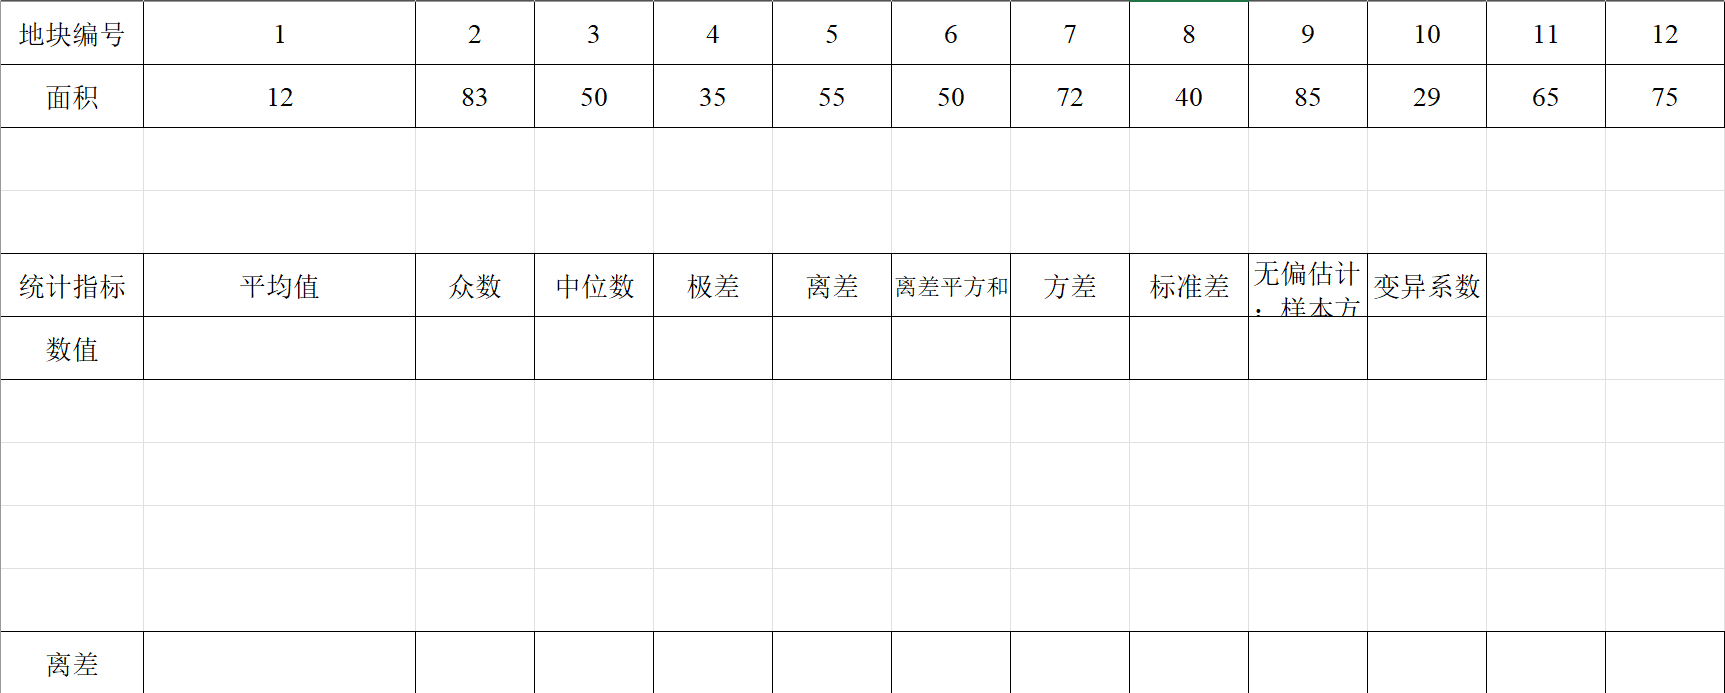
\includegraphics{../picture/exp1-1.png}

\begin{Shaded}
\begin{Highlighting}[]
\CommentTok{\# 定义计算函数}
\NormalTok{comstatindic }\OtherTok{=}\NormalTok{ \textbackslash{}(x)\{}
\NormalTok{  meanx }\OtherTok{=} \FunctionTok{mean}\NormalTok{(x)}
\NormalTok{  u }\OtherTok{=} \FunctionTok{unique}\NormalTok{(x)}
\NormalTok{  tab }\OtherTok{=} \FunctionTok{tabulate}\NormalTok{(}\FunctionTok{match}\NormalTok{(x, u))}
\NormalTok{  modex }\OtherTok{=}\NormalTok{ u[tab }\SpecialCharTok{==} \FunctionTok{max}\NormalTok{(tab)]}
\NormalTok{  medianx }\OtherTok{=} \FunctionTok{median}\NormalTok{(x)}
\NormalTok{  rangex }\OtherTok{=} \FunctionTok{max}\NormalTok{(x) }\SpecialCharTok{{-}} \FunctionTok{min}\NormalTok{(x)}
\NormalTok{  deviationx }\OtherTok{=}\NormalTok{ x }\SpecialCharTok{{-}}\NormalTok{ meanx}
\NormalTok{  squre\_deviationx }\OtherTok{=} \FunctionTok{sum}\NormalTok{(deviationx }\SpecialCharTok{\^{}} \DecValTok{2}\NormalTok{)}
\NormalTok{  variancex }\OtherTok{=}\NormalTok{ squre\_deviationx }\SpecialCharTok{/} \FunctionTok{length}\NormalTok{(x)}
\NormalTok{  sdx }\OtherTok{=} \FunctionTok{sqrt}\NormalTok{(variancex)}
\NormalTok{  unbias\_sdx }\OtherTok{=} \FunctionTok{sqrt}\NormalTok{(squre\_deviationx }\SpecialCharTok{/}\NormalTok{ (}\FunctionTok{length}\NormalTok{(x) }\SpecialCharTok{{-}} \DecValTok{1}\NormalTok{))}
\NormalTok{  cvx }\OtherTok{=}\NormalTok{ unbias\_sdx }\SpecialCharTok{/}\NormalTok{ meanx}
\NormalTok{  dt1 }\OtherTok{=} \FunctionTok{c}\NormalTok{(meanx,modex,medianx,rangex,squre\_deviationx,}
\NormalTok{          variancex,sdx,unbias\_sdx,cvx)}
  \FunctionTok{names}\NormalTok{(dt1) }\OtherTok{=} \FunctionTok{c}\NormalTok{(}\StringTok{"平均值"}\NormalTok{,}\StringTok{"众数"}\NormalTok{,}\StringTok{"中位数"}\NormalTok{,}\StringTok{"极差"}\NormalTok{,}\StringTok{"离差平方和"}\NormalTok{,}
                 \StringTok{"方差"}\NormalTok{,}\StringTok{"标准差"}\NormalTok{,}\StringTok{"标准差的无偏估计"}\NormalTok{,}\StringTok{"变异系数"}\NormalTok{)}
  \FunctionTok{return}\NormalTok{(}\FunctionTok{list}\NormalTok{(dt1,}\StringTok{"离差"} \OtherTok{=}\NormalTok{ deviationx))}
\NormalTok{\}}

\NormalTok{ug }\OtherTok{=} \FunctionTok{c}\NormalTok{(}\DecValTok{12}\NormalTok{,}\DecValTok{83}\NormalTok{,}\DecValTok{50}\NormalTok{,}\DecValTok{35}\NormalTok{,}\DecValTok{55}\NormalTok{,}\DecValTok{50}\NormalTok{,}\DecValTok{72}\NormalTok{,}\DecValTok{40}\NormalTok{,}\DecValTok{85}\NormalTok{,}\DecValTok{29}\NormalTok{,}\DecValTok{65}\NormalTok{,}\DecValTok{75}\NormalTok{)}
\FunctionTok{comstatindic}\NormalTok{(ug)}
\end{Highlighting}
\end{Shaded}

\begin{verbatim}
## [[1]]
##           平均值             众数           中位数             极差 
##       54.2500000       50.0000000       52.5000000       73.0000000 
##       离差平方和             方差           标准差 标准差的无偏估计 
##     5666.2500000      472.1875000       21.7298757       22.6961150 
##         变异系数 
##        0.4183616 
## 
## $离差
##  [1] -42.25  28.75  -4.25 -19.25   0.75  -4.25  17.75 -14.25  30.75 -25.25
## [11]  10.75  20.75
\end{verbatim}

\subsection{分组数据平均值,中位数,众数的计算}

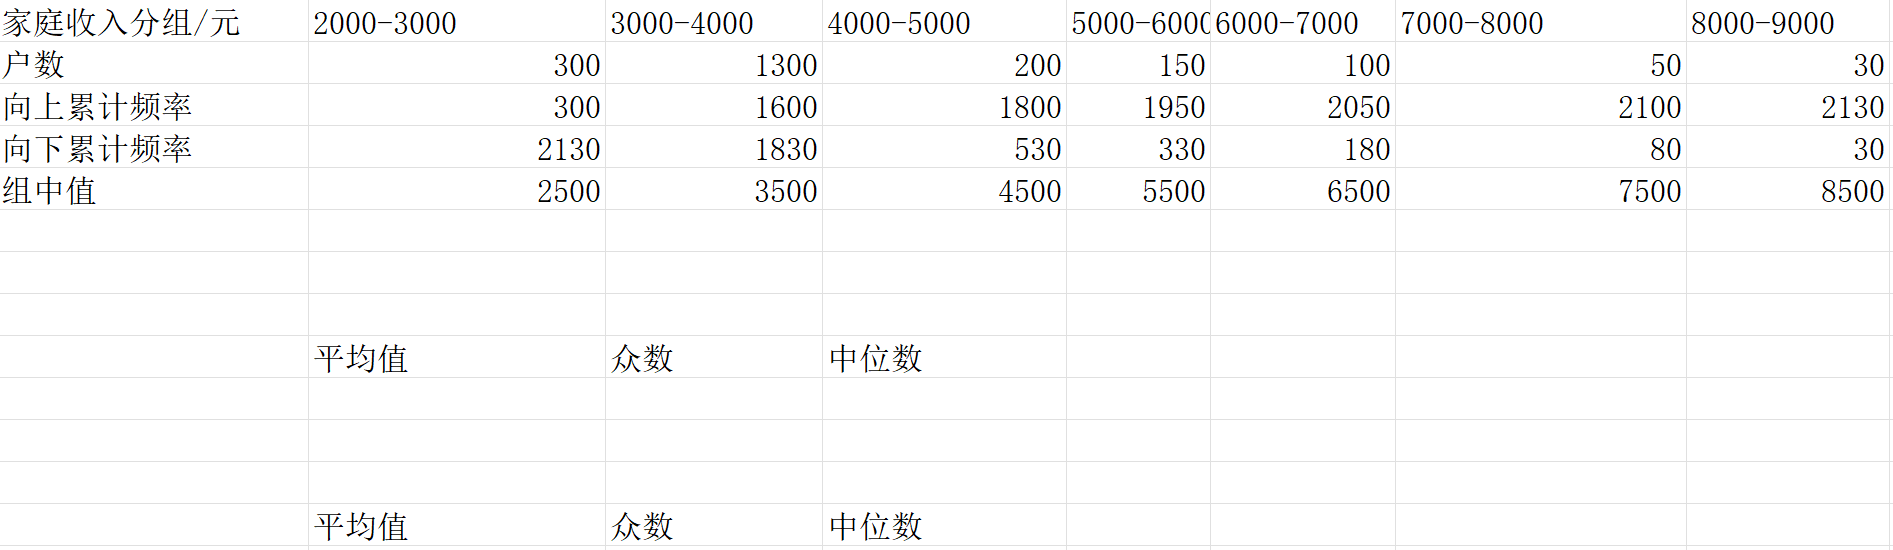
\includegraphics{../picture/exp1-2.png}

\begin{Shaded}
\begin{Highlighting}[]
\CommentTok{\# 首先构造输入数据}
\NormalTok{g }\OtherTok{=}\NormalTok{ tibble}\SpecialCharTok{::}\FunctionTok{tibble}\NormalTok{(}
\NormalTok{  家庭收入分组 }\OtherTok{=} \FunctionTok{paste}\NormalTok{(}\FunctionTok{seq}\NormalTok{(}\DecValTok{2000}\NormalTok{,}\DecValTok{8000}\NormalTok{,}\AttributeTok{by =} \DecValTok{1000}\NormalTok{),}
                       \FunctionTok{seq}\NormalTok{(}\DecValTok{3000}\NormalTok{,}\DecValTok{9000}\NormalTok{,}\AttributeTok{by =} \DecValTok{1000}\NormalTok{),}
                       \AttributeTok{sep =} \StringTok{"{-}"}\NormalTok{),}
\NormalTok{  户数 }\OtherTok{=} \FunctionTok{c}\NormalTok{(}\DecValTok{300}\NormalTok{,}\DecValTok{1300}\NormalTok{,}\DecValTok{200}\NormalTok{,}\DecValTok{150}\NormalTok{,}\DecValTok{100}\NormalTok{,}\DecValTok{50}\NormalTok{,}\DecValTok{30}\NormalTok{),}
\NormalTok{  向上累计频率 }\OtherTok{=} \FunctionTok{c}\NormalTok{(}\DecValTok{300}\NormalTok{,}\DecValTok{1600}\NormalTok{,}\DecValTok{1800}\NormalTok{,}\DecValTok{1950}\NormalTok{,}\DecValTok{2050}\NormalTok{,}\DecValTok{2100}\NormalTok{,}\DecValTok{2130}\NormalTok{),}
\NormalTok{  向下累计频率 }\OtherTok{=} \FunctionTok{c}\NormalTok{(}\DecValTok{2130}\NormalTok{,}\DecValTok{1830}\NormalTok{,}\DecValTok{530}\NormalTok{,}\DecValTok{330}\NormalTok{,}\DecValTok{180}\NormalTok{,}\DecValTok{80}\NormalTok{,}\DecValTok{30}\NormalTok{),}
\NormalTok{  组中值 }\OtherTok{=} \FunctionTok{c}\NormalTok{(}\DecValTok{2500}\NormalTok{,}\DecValTok{3500}\NormalTok{,}\DecValTok{4500}\NormalTok{,}\DecValTok{5500}\NormalTok{,}\DecValTok{6500}\NormalTok{,}\DecValTok{7500}\NormalTok{,}\DecValTok{8500}\NormalTok{)}
\NormalTok{)}
\NormalTok{g}
\end{Highlighting}
\end{Shaded}

\begin{verbatim}
## # A tibble: 7 x 5
##   家庭收入分组  户数 向上累计频率 向下累计频率 组中值
##   <chr>        <dbl>        <dbl>        <dbl>  <dbl>
## 1 2000-3000      300          300         2130   2500
## 2 3000-4000     1300         1600         1830   3500
## 3 4000-5000      200         1800          530   4500
## 4 5000-6000      150         1950          330   5500
## 5 6000-7000      100         2050          180   6500
## 6 7000-8000       50         2100           80   7500
## 7 8000-9000       30         2130           30   8500
\end{verbatim}

\paragraph{平均值计算}

\[
 \overline{x} = \frac{\sum\limits_{i=1}^{m}f_i x_i}{\sum\limits_{i=1}^{m}f_i}
\]

\(x_i(i = 1,2,\ldots,m)\)代表第\(i\)组的组中值,如果第\(i\)组的下限值为\(a_i\),
上限值为\(b_i\),则\(x_i = a_i + \frac{(b_i - a_i)}{2}\);
\(f_i\)代表第\(i\)组的频数,\(m\)为分组个数。

\begin{Shaded}
\begin{Highlighting}[]
\CommentTok{\# 计算分组数据的平均值}
\NormalTok{meang }\OtherTok{=} \FunctionTok{sum}\NormalTok{(g}\SpecialCharTok{$}\StringTok{\textasciigrave{}}\AttributeTok{组中值}\StringTok{\textasciigrave{}} \SpecialCharTok{*}\NormalTok{ g}\SpecialCharTok{$}\StringTok{\textasciigrave{}}\AttributeTok{户数}\StringTok{\textasciigrave{}}\NormalTok{) }\SpecialCharTok{/} \FunctionTok{sum}\NormalTok{(g}\SpecialCharTok{$}\StringTok{\textasciigrave{}}\AttributeTok{户数}\StringTok{\textasciigrave{}}\NormalTok{)}
\FunctionTok{cat}\NormalTok{(}\StringTok{"分组数据平均值为"}\NormalTok{,meang)}
\end{Highlighting}
\end{Shaded}

\begin{verbatim}
## 分组数据平均值为 3899.061
\end{verbatim}

\paragraph{众数计算}:

\textbf{法1}

\[
 M_o = L + d \times \frac{\Delta_1}{\Delta_1 + \Delta_2}
\]

\textbf{法2}

\[
 M_o = U - d \times \frac{\Delta_2}{\Delta_1 + \Delta_2}
\]

\(M_o\)为代求的分组数据的众数,\(L\)为众数所在组的下限值,\(U\)为众数所在组的上限值,\(\Delta_1\)为众数组频数与上一组频数之差,\(\Delta_2\)为众数组频数与下一组频数之差,\(d\)为众数所在组的组距

\begin{Shaded}
\begin{Highlighting}[]
\NormalTok{calcul\_mode }\OtherTok{=}\NormalTok{ \textbackslash{}(popn,floorn,ceiln)\{}
\NormalTok{  i }\OtherTok{=} \FunctionTok{match}\NormalTok{(}\FunctionTok{max}\NormalTok{(popn),popn)}
\NormalTok{  L }\OtherTok{=}\NormalTok{ floorn[i];U }\OtherTok{=}\NormalTok{ ceiln[i]}
\NormalTok{  delta1 }\OtherTok{=}\NormalTok{ popn[i] }\SpecialCharTok{{-}}\NormalTok{ popn[i}\DecValTok{{-}1}\NormalTok{]}
\NormalTok{  delta2 }\OtherTok{=}\NormalTok{ popn[i] }\SpecialCharTok{{-}}\NormalTok{ popn[i}\SpecialCharTok{+}\DecValTok{1}\NormalTok{]}
\NormalTok{  d }\OtherTok{=}\NormalTok{ U }\SpecialCharTok{{-}}\NormalTok{ L}
\NormalTok{  m1 }\OtherTok{=}\NormalTok{ L }\SpecialCharTok{+}\NormalTok{ d }\SpecialCharTok{*}\NormalTok{ delta1 }\SpecialCharTok{/}\NormalTok{ (delta1 }\SpecialCharTok{+}\NormalTok{ delta2)}
\NormalTok{  m2 }\OtherTok{=}\NormalTok{ U }\SpecialCharTok{{-}}\NormalTok{ d }\SpecialCharTok{*}\NormalTok{ delta2 }\SpecialCharTok{/}\NormalTok{ (delta1 }\SpecialCharTok{+}\NormalTok{ delta2)}
\NormalTok{  m }\OtherTok{=} \FunctionTok{c}\NormalTok{(m1,m2)}
  \FunctionTok{setNames}\NormalTok{(m,}\FunctionTok{c}\NormalTok{(}\StringTok{\textquotesingle{}法1计算的众数\textquotesingle{}}\NormalTok{,}\StringTok{\textquotesingle{}法2计算的众数\textquotesingle{}}\NormalTok{))}
\NormalTok{\}}

\NormalTok{xfloor }\OtherTok{=} \FunctionTok{seq}\NormalTok{(}\DecValTok{2000}\NormalTok{,}\DecValTok{8000}\NormalTok{,}\AttributeTok{by =} \DecValTok{1000}\NormalTok{)}
\NormalTok{xceil }\OtherTok{=}  \FunctionTok{seq}\NormalTok{(}\DecValTok{3000}\NormalTok{,}\DecValTok{9000}\NormalTok{,}\AttributeTok{by =} \DecValTok{1000}\NormalTok{)}
\NormalTok{xpop }\OtherTok{=}\NormalTok{ g}\SpecialCharTok{$}\StringTok{\textasciigrave{}}\AttributeTok{户数}\StringTok{\textasciigrave{}}
\NormalTok{modeg }\OtherTok{=} \FunctionTok{calcul\_mode}\NormalTok{(xpop,xfloor,xceil)}
\NormalTok{modeg}
\end{Highlighting}
\end{Shaded}

\begin{verbatim}
## 法1计算的众数 法2计算的众数 
##       3476.19       3476.19
\end{verbatim}

\paragraph{中位数计算}:

\textbf{法1}

\[
 M_e = L + d \times \frac{\frac{1}{2} \sum\limits_{i=1}^{n}f_i - S_{m - 1}}{f_m}
\]

\textbf{法2}

\[
 M_e = U - d \times \frac{\frac{1}{2} \sum\limits_{i=1}^{n}f_i - S_{m + 1}}{f_m}
\]

\(M_e\)为代求的分组数据的中位数,\(L\)为中位数所在组的下限值,\(U\)为中位数所在组的上限值,\(n\)为分组个数,\(f_i\)为第\(i\)组对应的频数,\(f_m\)为中位数所在组的频数,\(S_{m-1}\)为中位数所在组以下的累积频数,\(S_{m+1}\)为中位数所在组以上的累积频数,\(d\)为中位数所在组的组距

\begin{Shaded}
\begin{Highlighting}[]
\NormalTok{calcul\_median }\OtherTok{=}\NormalTok{ \textbackslash{}(popn,floorn,ceiln)\{}
\NormalTok{  halfpop }\OtherTok{=} \FunctionTok{sum}\NormalTok{(popn) }\SpecialCharTok{*} \FloatTok{0.5}
\NormalTok{  i }\OtherTok{=} \FunctionTok{which}\NormalTok{(}\FunctionTok{cumsum}\NormalTok{(popn) }\SpecialCharTok{{-}}\NormalTok{ halfpop }\SpecialCharTok{\textgreater{}} \DecValTok{0}\NormalTok{)[}\DecValTok{1}\NormalTok{]}
\NormalTok{  L }\OtherTok{=}\NormalTok{ floorn[i];U }\OtherTok{=}\NormalTok{ ceiln[i]}
\NormalTok{  d }\OtherTok{=}\NormalTok{ U }\SpecialCharTok{{-}}\NormalTok{ L}
\NormalTok{  fm }\OtherTok{=}\NormalTok{ popn[i]}
\NormalTok{  sms1 }\OtherTok{=} \FunctionTok{sum}\NormalTok{(popn[}\DecValTok{1}\SpecialCharTok{:}\NormalTok{(i}\DecValTok{{-}1}\NormalTok{)])}
\NormalTok{  sma1 }\OtherTok{=} \FunctionTok{sum}\NormalTok{(popn[(i}\SpecialCharTok{+}\DecValTok{1}\NormalTok{)}\SpecialCharTok{:}\FunctionTok{length}\NormalTok{(popn)])}
\NormalTok{  m1 }\OtherTok{=}\NormalTok{ L }\SpecialCharTok{+}\NormalTok{ d }\SpecialCharTok{*}\NormalTok{ (halfpop }\SpecialCharTok{{-}}\NormalTok{ sms1) }\SpecialCharTok{/}\NormalTok{ fm}
\NormalTok{  m2 }\OtherTok{=}\NormalTok{ U }\SpecialCharTok{{-}}\NormalTok{ d }\SpecialCharTok{*}\NormalTok{ (halfpop }\SpecialCharTok{{-}}\NormalTok{ sma1) }\SpecialCharTok{/}\NormalTok{ fm}
\NormalTok{  m }\OtherTok{=} \FunctionTok{c}\NormalTok{(m1,m2)}
  \FunctionTok{setNames}\NormalTok{(m,}\FunctionTok{c}\NormalTok{(}\StringTok{\textquotesingle{}法1计算的中位数\textquotesingle{}}\NormalTok{,}\StringTok{\textquotesingle{}法2计算的中位数\textquotesingle{}}\NormalTok{))}
\NormalTok{\}}

\NormalTok{xfloor }\OtherTok{=} \FunctionTok{seq}\NormalTok{(}\DecValTok{2000}\NormalTok{,}\DecValTok{8000}\NormalTok{,}\AttributeTok{by =} \DecValTok{1000}\NormalTok{)}
\NormalTok{xceil }\OtherTok{=}  \FunctionTok{seq}\NormalTok{(}\DecValTok{3000}\NormalTok{,}\DecValTok{9000}\NormalTok{,}\AttributeTok{by =} \DecValTok{1000}\NormalTok{)}
\NormalTok{xpop }\OtherTok{=}\NormalTok{ g}\SpecialCharTok{$}\StringTok{\textasciigrave{}}\AttributeTok{户数}\StringTok{\textasciigrave{}}
\NormalTok{mediang }\OtherTok{=} \FunctionTok{calcul\_median}\NormalTok{(xpop,xfloor,xceil)}
\NormalTok{mediang}
\end{Highlighting}
\end{Shaded}

\begin{verbatim}
## 法1计算的中位数 法2计算的中位数 
##        3588.462        3588.462
\end{verbatim}

所以分组数据的平均值为3899.0610329,众数为3476.1904762,中位数为3588.4615385.

\end{document}
